% =========================================================
% PART I -- FOUNDATIONS
% =========================================================

\section{Foundations}

% ---------------------------------------------------------
% 1. STATISTICS
% ---------------------------------------------------------

\begin{frame}{1. Statistics}

\textbf{Definition}

Statistics is the science of collecting, organizing, summarizing,
analyzing, interpreting, and presenting data to obtain meaningful
information and support decision-making.

\vspace{0.4cm}

\textbf{Main branches}

\begin{itemize}
    \item \textbf{Descriptive Statistics} -- summarizes and presents data.
    \item \textbf{Inferential Statistics} -- uses sample data to draw
    conclusions about a population.
\end{itemize}

\vspace{0.3cm}

\textbf{Example}

For the marks of 50 students, calculating the mean and standard
deviation describes the data, while using the sample to estimate
the average marks of the entire class is an inferential task.

\end{frame}


% ---------------------------------------------------------
% 2. DATA
% ---------------------------------------------------------

\begin{frame}{2. Data}

\textbf{Definition}

Data are raw facts, observations, measurements, or values collected
for analysis.

\textbf{Examples}

\begin{itemize}
    \item Student marks: $72, 85, 64, 91$
    \item Age: $20, 21, 22, 20$
    \item Temperature: $28.5^\circ C$
    \item Image pixels represented by numerical values
\end{itemize}

\textbf{Mathematical Representation}

A dataset can be represented as

\[
X = \{x_1,x_2,\ldots,x_n\}
\]

where $x_i$ represents an observation and $n$ is the number of
observations.

\textbf{Application:} Data forms the basic input for statistical
analysis and machine learning models.

\end{frame}


% ---------------------------------------------------------
% 3. INFORMATION
% ---------------------------------------------------------

\begin{frame}{3. Information}

\textbf{Definition}

Information is processed, organized, and interpreted data that
provides meaning.

\textbf{Example}

Suppose the marks are \[
60,\;70,\;80,\;90,\;100
\]

The raw values are \textbf{data}.

Their average, \[
\bar{x} = 80,
\]

provides meaningful information about the overall performance.

\textbf{Key idea}

\[
\boxed{\text{Data} \longrightarrow \text{Processing} 
\longrightarrow \text{Information}}
\]

\end{frame}


% ---------------------------------------------------------
% 4. KNOWLEDGE
% ---------------------------------------------------------

\begin{frame}{4. Knowledge}

\textbf{Definition}

Knowledge is the understanding obtained from information by
identifying relationships, patterns, rules, or meaningful insights.

\vspace{0.4cm}

\textbf{Example}

If analysis shows that students who regularly attend classes
generally obtain higher marks, this observed relationship contributes
to knowledge.

\vspace{0.4cm}

\textbf{Flow}
\[
\text{Data}
\rightarrow
\text{Information}
\rightarrow
\text{Knowledge}
\]

\vspace{0.3cm}

\textbf{Application}

In computing and AI, knowledge can be used to build rules,
models, and systems that support prediction and decision-making.

\end{frame}


% ---------------------------------------------------------
% 5. INTELLIGENCE
% ---------------------------------------------------------

\begin{frame}{5. Intelligence}

\textbf{Definition}

Intelligence is the ability to use knowledge to learn, reason,
solve problems, make decisions, and adapt to new situations.

\vspace{0.4cm}

\textbf{Example}

A machine learning system can:

\begin{enumerate}
    \item Learn patterns from data.
    \item Convert patterns into useful information.
    \item Build knowledge from these patterns.
    \item Use the learned knowledge to make predictions or decisions.
\end{enumerate}

\vspace{0.4cm}

\textbf{Conceptual Flow}

\[
\boxed{
\text{Data}
\rightarrow
\text{Information}
\rightarrow
\text{Knowledge}
\rightarrow
\text{Intelligence}
}
\]

\end{frame}


% ---------------------------------------------------------
% 6. TYPES OF DATA
% ---------------------------------------------------------

\begin{frame}{6. Types of Data}

Data can be classified according to the number of variables
being observed.

\vspace{0.3cm}

\begin{block}{Univariate Data}
Data involving \textbf{one variable}.
\end{block}

\begin{block}{Bivariate Data}
Data involving \textbf{two variables}, often used to study their
relationship.
\end{block}

\begin{block}{Multivariate Data}
Data involving \textbf{three or more variables}.
\end{block}

\end{frame}


% ---------------------------------------------------------
% UNIVARIATE
% ---------------------------------------------------------

\begin{frame}{6.1 Univariate Data}

\textbf{Definition}

Univariate data contains observations of a single variable.

\textbf{Example}

Heights of five students:
\[
X = \{160,165,170,172,168\}
\]

Here, the only variable is \textbf{height}.

\textbf{Common analysis}

\begin{itemize}
    \item Mean
    \item Median
    \item Mode
    \item Variance
    \item Standard deviation

\end{itemize}

\textbf{Application:} Used to understand the distribution and
variability of a single feature.

\end{frame}


% ---------------------------------------------------------
% BIVARIATE
% ---------------------------------------------------------

\begin{frame}{6.2 Bivariate Data}

\textbf{Definition}

Bivariate data contains observations of two variables measured
on the same subjects.

\textbf{Example}

Consider years of education and income:
\[
X = \text{Years of Education}, \qquad
Y = \text{Income}
\]
Each observation is represented as a pair
\[
(x_i,y_i).
\]

\textbf{Common analysis}

\begin{itemize}
    \item Covariance
    \item Correlation
    \item Simple linear regression
\end{itemize}

\textbf{Application:} Used to study relationships between two
variables.

\end{frame}

% ---------------------------------------------------------
% 6.2 BIVARIATE DATA -- FIGURE
% ---------------------------------------------------------

\begin{frame}{6.2 Bivariate Data -- Figure}

\begin{columns}[T]

\begin{column}{0.55\textwidth}

\centering
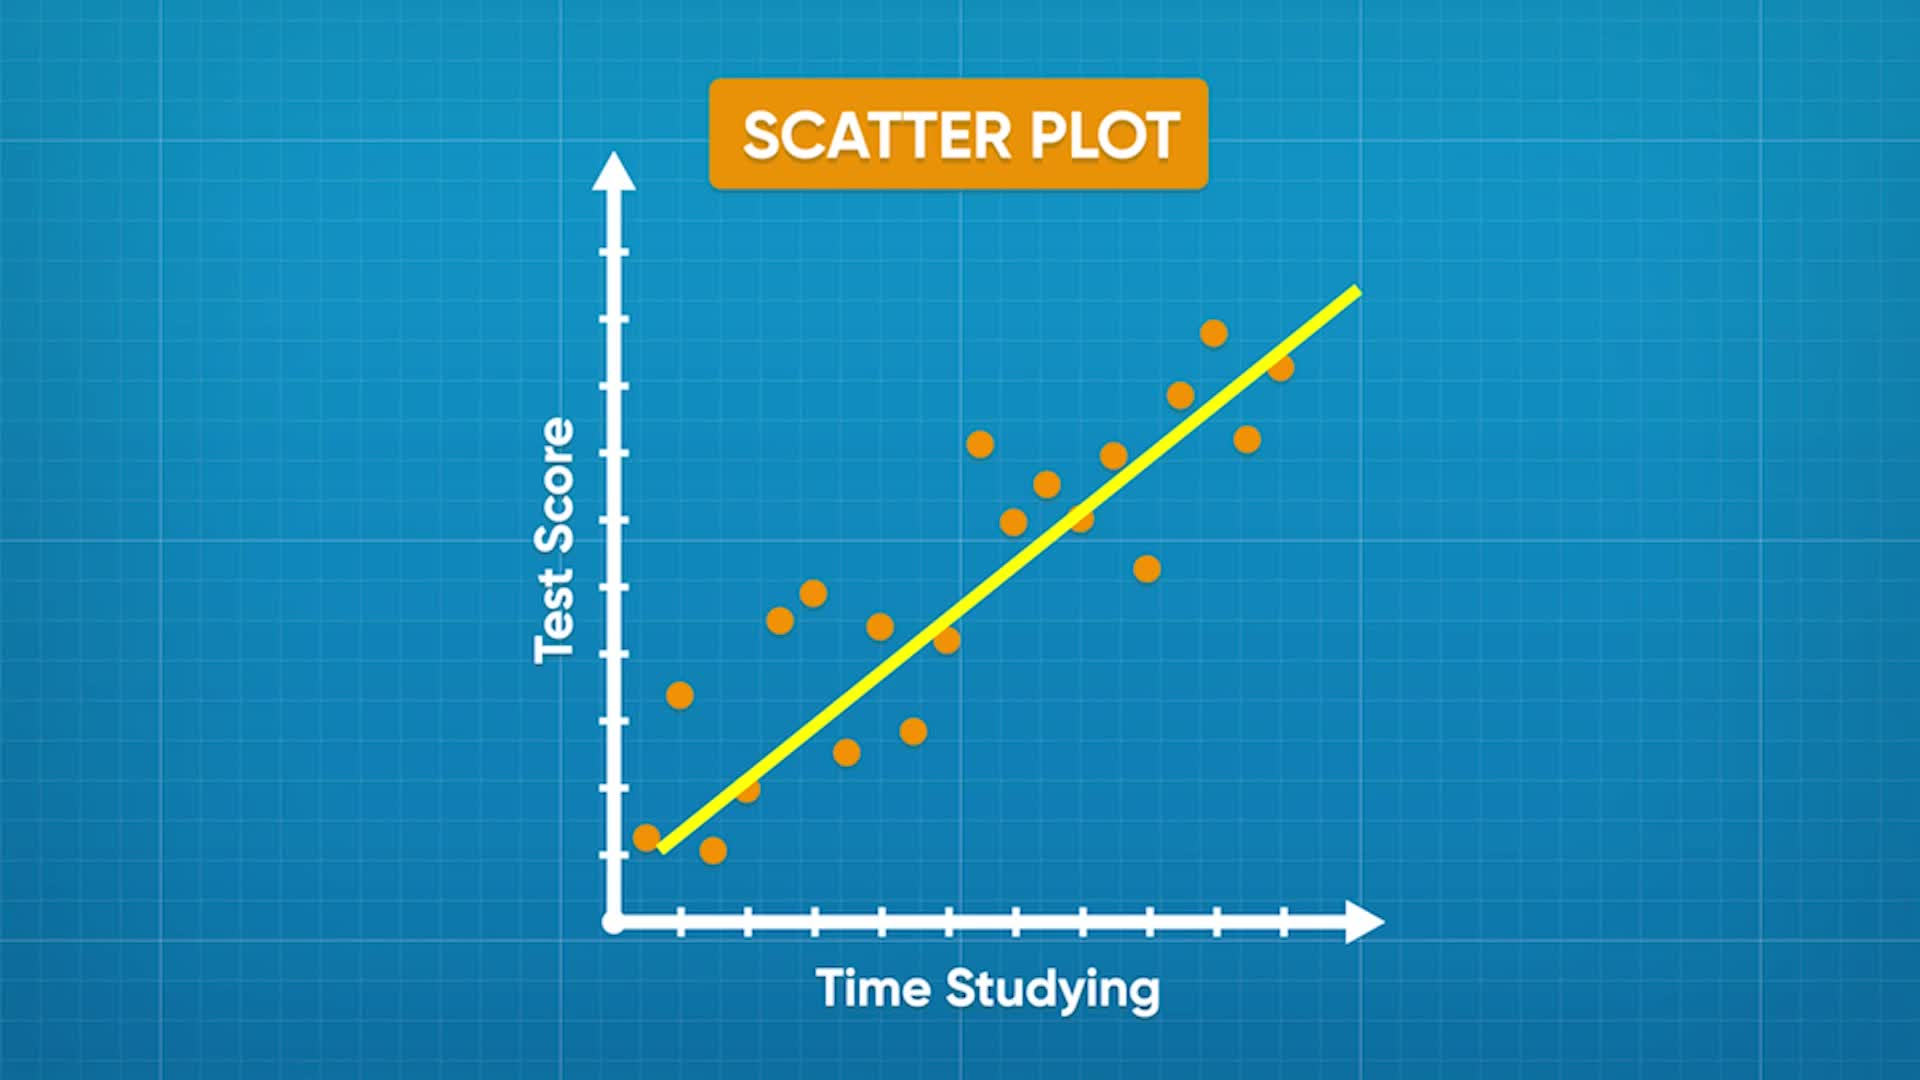
\includegraphics[width=\textwidth]{figures/bivariate.jpg}

\end{column}

\begin{column}{0.42\textwidth}

The figure represents bivariate data by showing the
relationship between two variables.

\vspace{0.3cm}

Each point represents one observation with a value for
both variables.

\vspace{0.3cm}

\textbf{Key Observation}

The pattern of the points helps us identify whether the
two variables have a possible relationship.

\end{column}

\end{columns}

\end{frame}

% ---------------------------------------------------------
% MULTIVARIATE
% ---------------------------------------------------------

\begin{frame}{6.3 Multivariate Data}

\textbf{Definition}

Multivariate data contains observations involving three or more
variables.

\textbf{Example} A student dataset may contain:
\[
\{\text{Age, Attendance, Study Hours, Marks}\}
\]
Each observation can be represented as
\[
\mathbf{x}_i =
(x_{i1},x_{i2},\ldots,x_{ip})
\]
where $p$ is the number of variables.

\textbf{Common analysis}

\begin{itemize}
    \item Covariance matrix
    \item Correlation analysis
    \item Multiple regression
\end{itemize}

\textbf{Application:} Most real-world AI and machine learning
datasets are multivariate.

\end{frame}

% ---------------------------------------------------------
% 6.3 MULTIVARIATE DATA -- FIGURE
% ---------------------------------------------------------

\begin{frame}{6.3 Multivariate Data -- Figure}

\begin{columns}[T]

\begin{column}{0.58\textwidth}

\centering
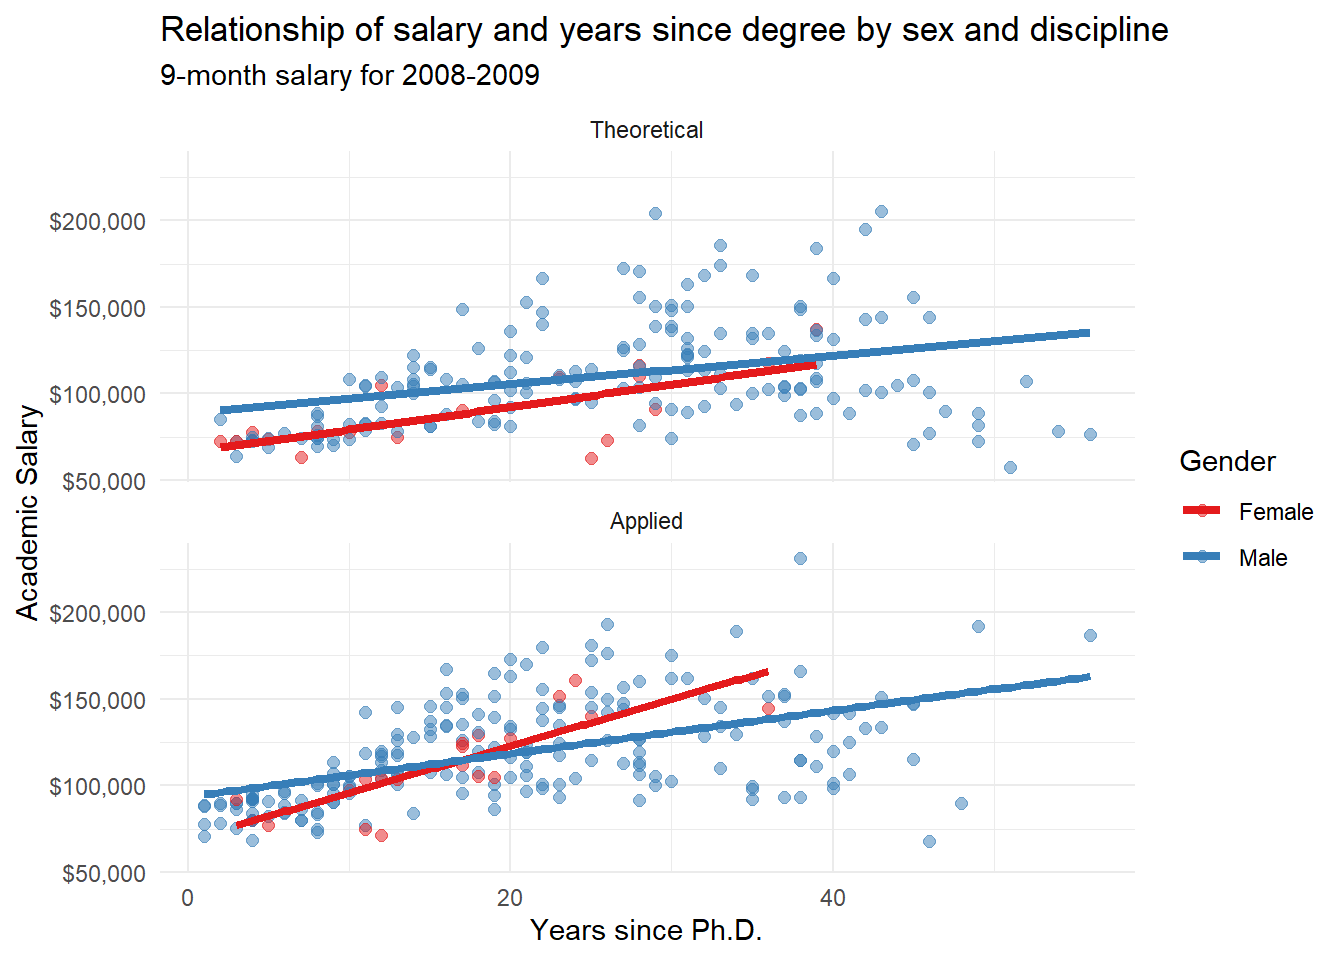
\includegraphics[width=\textwidth]{figures/multivariate.png}

\end{column}

\begin{column}{0.38\textwidth}

The figure represents data involving more than
two variables simultaneously. Each observation
contains multiple measurements.

\vspace{0.4cm}

\textbf{Observation}

The figure shows how several variables can be
examined together to identify patterns and
relationships in the data.

\end{column}

\end{columns}

\end{frame}